\chapter{Experimental setup}
\label{chap:detector}
%20-25 pages.
Intro to chapter.

\section{The Large Hadron Collider}
%CERN and LHC. Franco-Swiss border. 26 km. 100m underground. 
%Largest and most powerful.
The LHC at CERN is a circular accelerator and collider of protons (and lead 
ions). It is 27~kilometres in circumference, and is situated on the border 
between France and Switzerland near Geneva, approximately 100~metres 
underground. It was designed to investigate the standard model and search for 
new physics. The Higgs boson was successfully discovered at the LHC in 
2012~\cite{higgs-cms,higgs-atlas}.

\begin{figure}
\centering
% trim={left bottom right top}
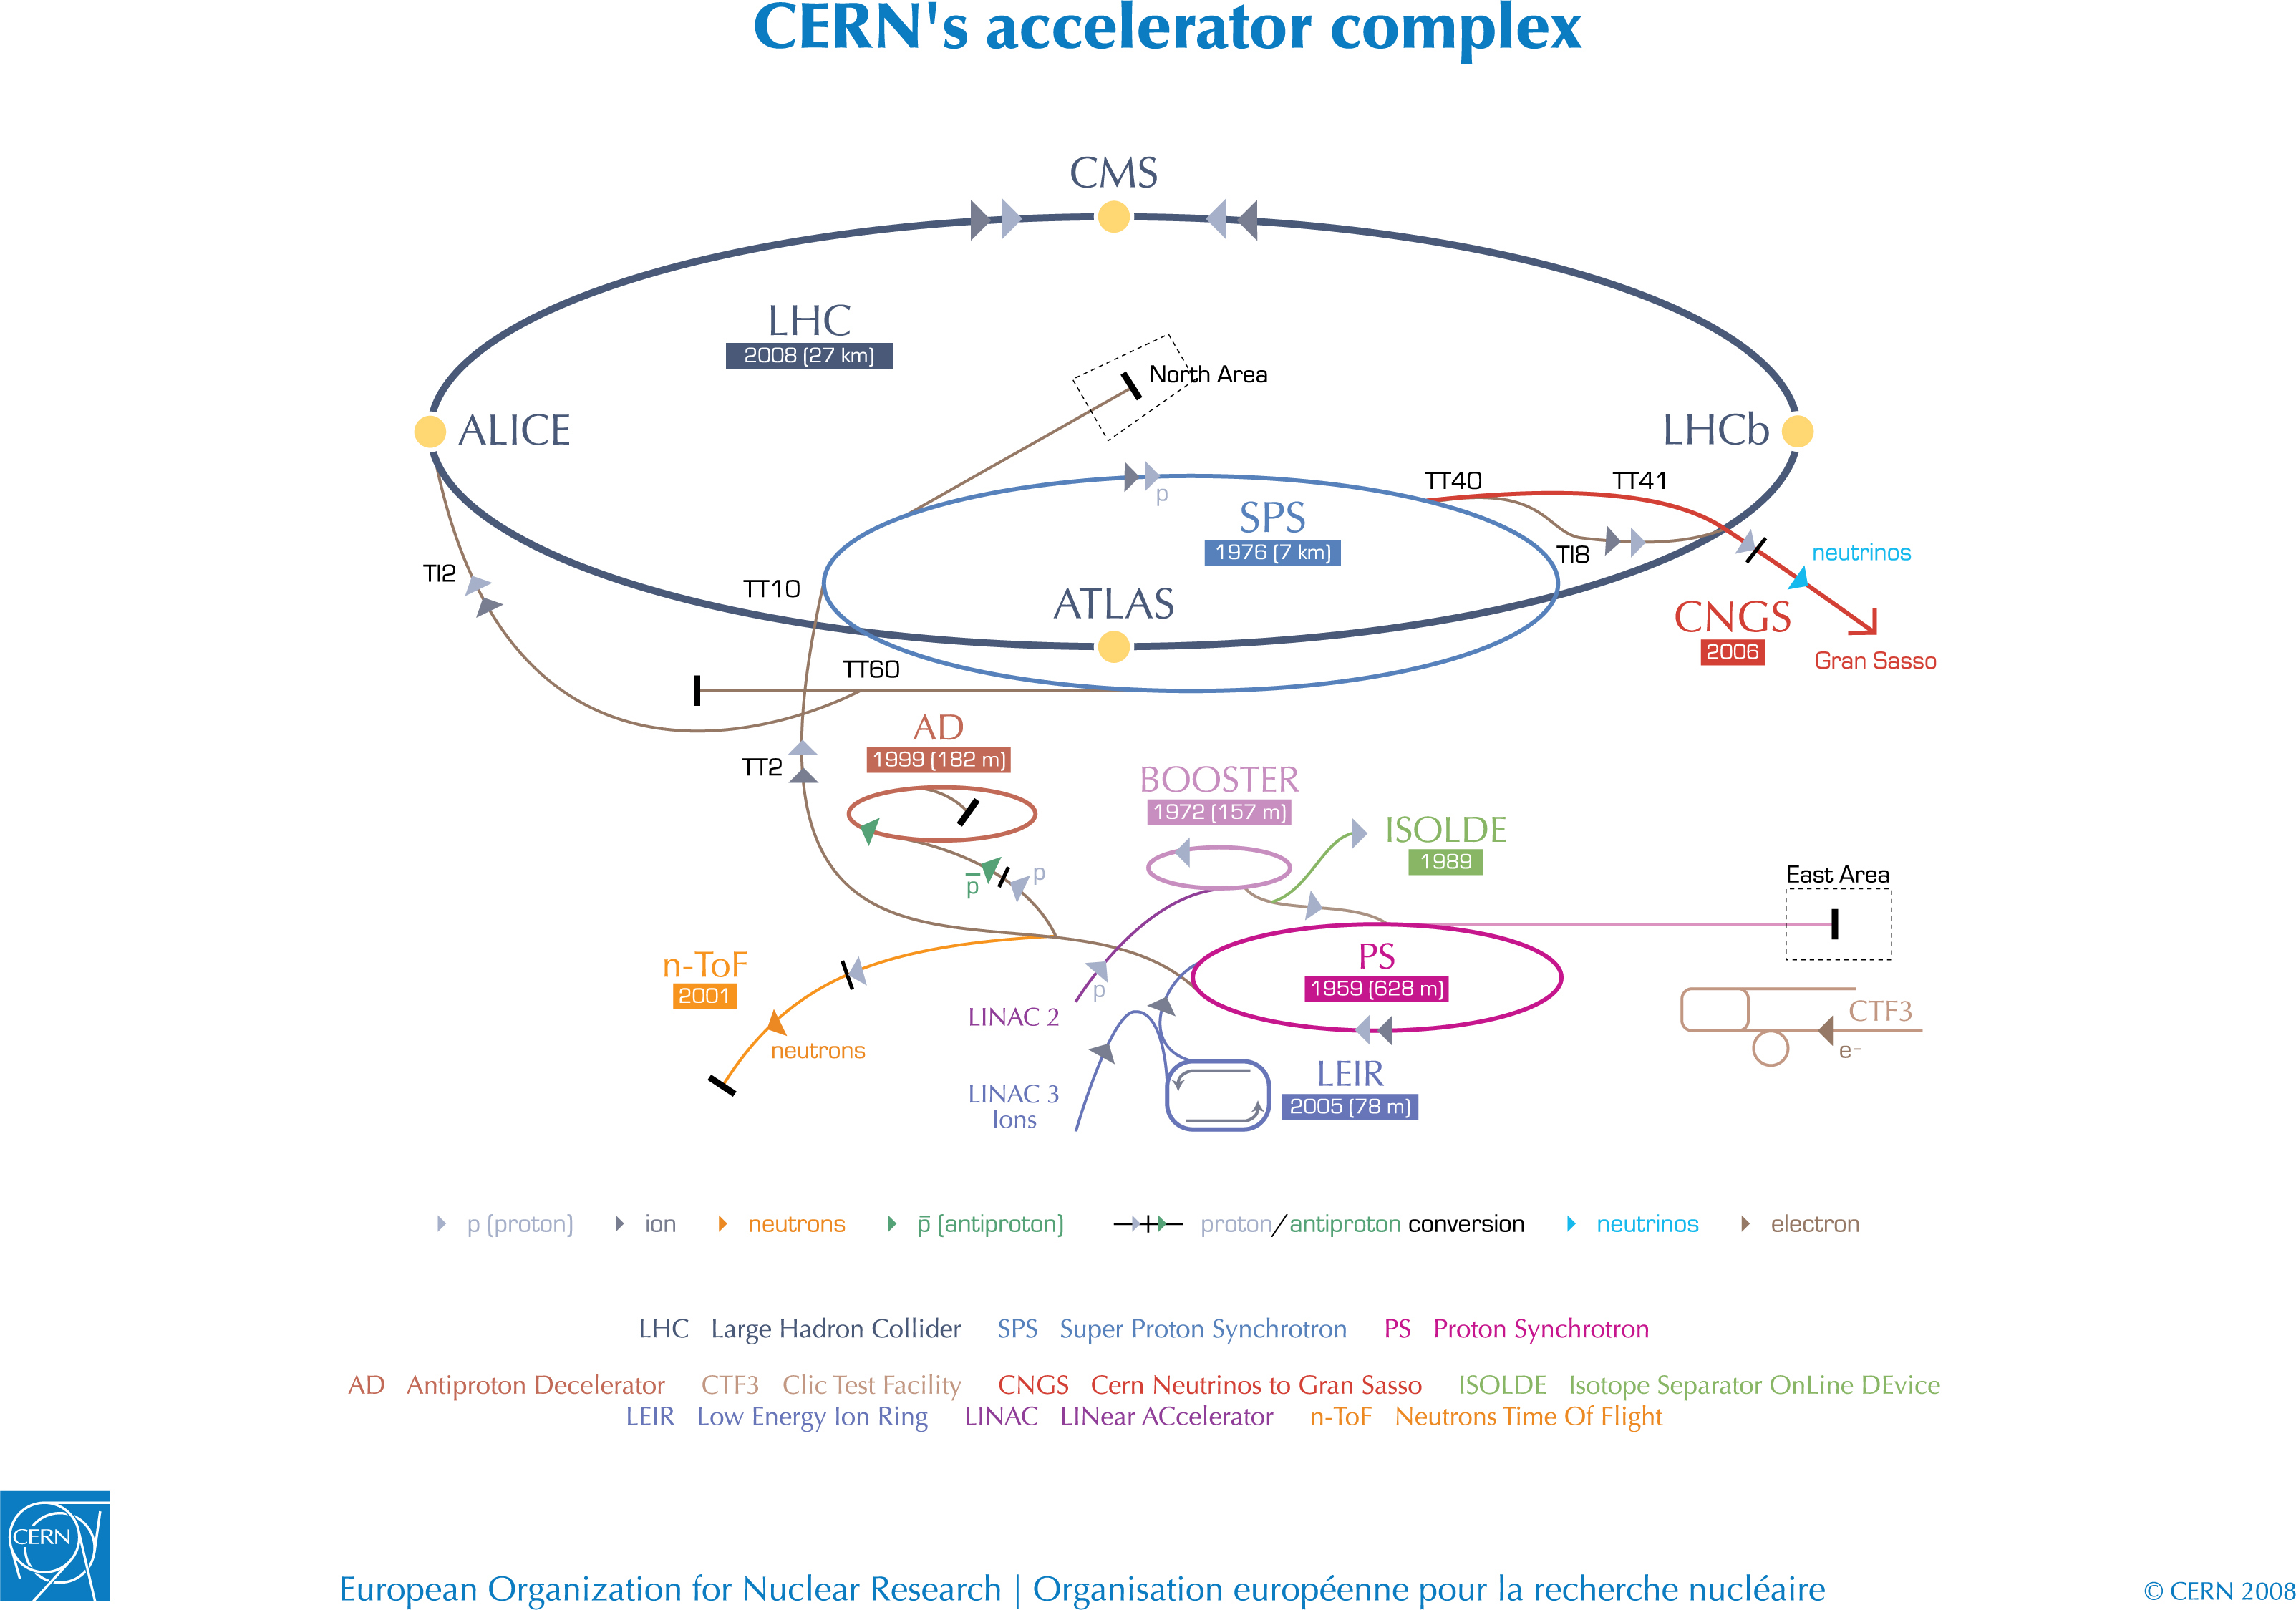
\includegraphics[width=1\textwidth, trim={2cm 5cm 2cm 1.5cm}, 
clip]{figs/detector/lhc-complex}
\caption{The accelerator complex at CERN leading to the LHC~\cite{lhc-complex}. 
The various accelerators (LINAC 2, PSB, PS, SPS, LHC) and detectors (CMS, 
ATLAS, LHCb, ALICE) are described in the text.}
\label{fig:lhc-complex}
\end{figure}

%Accelerator complex: hydrogen, LINAC, PS, SPS, etc (show diagram).
%4 detectors/collision points.
The accelerator complex at CERN is illustrated in Fig.~\ref{fig:lhc-complex}. 
The particle acceleration occurs in various stages. First, hydrogen atoms from 
a gas bottle are stripped of their electrons and the resulting protons are 
accelerated to 50~MeV in the Linear Accelerator 2 (LINAC 2). These protons are 
then injected into the Proton Synchrotron Booster (PSB) to increase their 
energy to 1.4~GeV. This is followed by the Proton Synchrotron (PS), where the 
protons reach 25~GeV, and the Super Proton Synchrotron (SPS), which further 
accelerates them to 450~GeV. The protons then finally arrive at the LHC, where 
they are accelerated by radio frequency cavities up to an energy of 6.5~TeV, 
and are steered and focussed by superconducting magnets.
% dipole to steer, quadrupole to focus
% 1200 dipole magnets, 8 Tesla
% https://home.cern/about/engineering/radiofrequency-cavities
During this process, the protons are also collected into bunches of 
approximately 115~billion protons each that are 25~ns apart. The total number 
of proton bunches circulating within a given fill of the LHC is 2808.
% bunches are 30 cm long
% spatial separation is 7.5 m 

The LHC consists of two beam pipes in which the protons are circulated in 
opposite directions. The protons are made to collide at a centre of mass energy 
of 13~TeV at four points on the ring, where the CMS~\cite{cms}, 
ATLAS~\cite{atlas}, LHCb~\cite{lhcb} and ALICE~\cite{alice} detectors are 
situated. CMS and ATLAS are both general purpose detectors, while LHCb and 
ALICE are focussed on b-physics and heavy ion physics, respectively.
% CP violation via the decays of b hadrons

For a process with a production cross section $\sigma$, the expected number of 
events per unit time is related to the instantaneous luminosity $L$ by the 
relation:
\begin{equation}
\frac{\mathrm d N}{\mathrm d t} = \sigma L \, .
\end{equation}
The instantaneous luminosity is proportional to the number of proton bunches, 
the number of protons per bunch and the revolution frequency, and is inversely 
proportional to the transverse size of the beam~\cite{pdg12}. 
% transverse dimensions are 15 microns
For the 2016 running conditions, the average instantaneous luminosity of the 
LHC was approximately $10^{34}$~\lumiunits, which resulted in an average number 
of 
interactions per bunch crossing (referred to as pileup) of $\sim$20.
% plug in inelastic xs to get pileup events per ns, multiply by 25 (50) to get 
%pileup events per bunch crossing
The total expected number of events of a process in a certain time $T$ is given 
by:
\begin{equation}
N = \sigma \int_{0}^{T} L \mathrm d t = \sigma L_\mathrm{int} \, ,
\end{equation}
where the integral of the instantaneous luminosity over this time is called the 
integrated luminosity $L_\mathrm{int}$, and is a measure of the amount of data 
collected.

%Luminosity (instantaneous/integrated) and cross section formulas 
%(Marco-Andrea/Pesaresi).
%Pileup 20 (formula/estimate using inelastic xs?). Minimum bias.
%Bunch spacing, number of bunches, number of protons per bunch (Marco-Andrea 
%table).
%History of Run1, shutdown, Run 2. Amount of data delivered.

\begin{comment}
Collider physics.
Used to search for new physics and discover Higgs boson.
Need very high energy to produce high mass particles and search for new physics 
(cf xs vs com).
(Compare to ep collider and fixed target).
Proton-proton (and ion) collisions.
Centre of mass energy. 
Describe run, fill, lumi section, instantaneous luminosity values.
\end{comment}

\section{The Compact Muon Solenoid}
%One of two multipurpose detectors. Used to search for new physics and discover 
%Higgs boson.
%Hermetic coverage (good for MET). 
%identify particles (electrons, photons, hadrons, muons) with high precision
% Give size and mass? MA: 22 meters long and about 15 meters in diameter, with 
%a weight of 12,500 metric tons [55]. Isn't it 14,000 tonnes? The complete 
%detector is 21 metres long, 15 metres wide and 15 metres high.
The CMS detector is one of the two general purpose detectors at the LHC along 
with ATLAS, and was designed with the main goal of searching for the Higgs 
boson as well as new physics beyond the standard model. The detector is 
cylindrical 
and consists of several layers of subdetectors and a solenoid magnet that are 
used to track, identify and measure the energy of particles such as electrons, 
photons, muons and hadrons. 
It extends up to a pseudorapidity of $\etaabs \approx 5$, providing an almost 
complete coverage in solid angle. This is important when reconstructing the 
momentum of a weakly interacting particle via the `missing momentum' in an 
event.
The detector is approximately 22~m in length and 15~m in diameter, and weighs 
about 14,000 tonnes.
The layout of the CMS detector is shown in Fig.~\ref{fig:cms3d}, and a 
cross-sectional view is given in Fig.~\ref{fig:cms2d}, illustrating the various 
components of the detector, which will be described in this section.

\begin{figure}
\centering
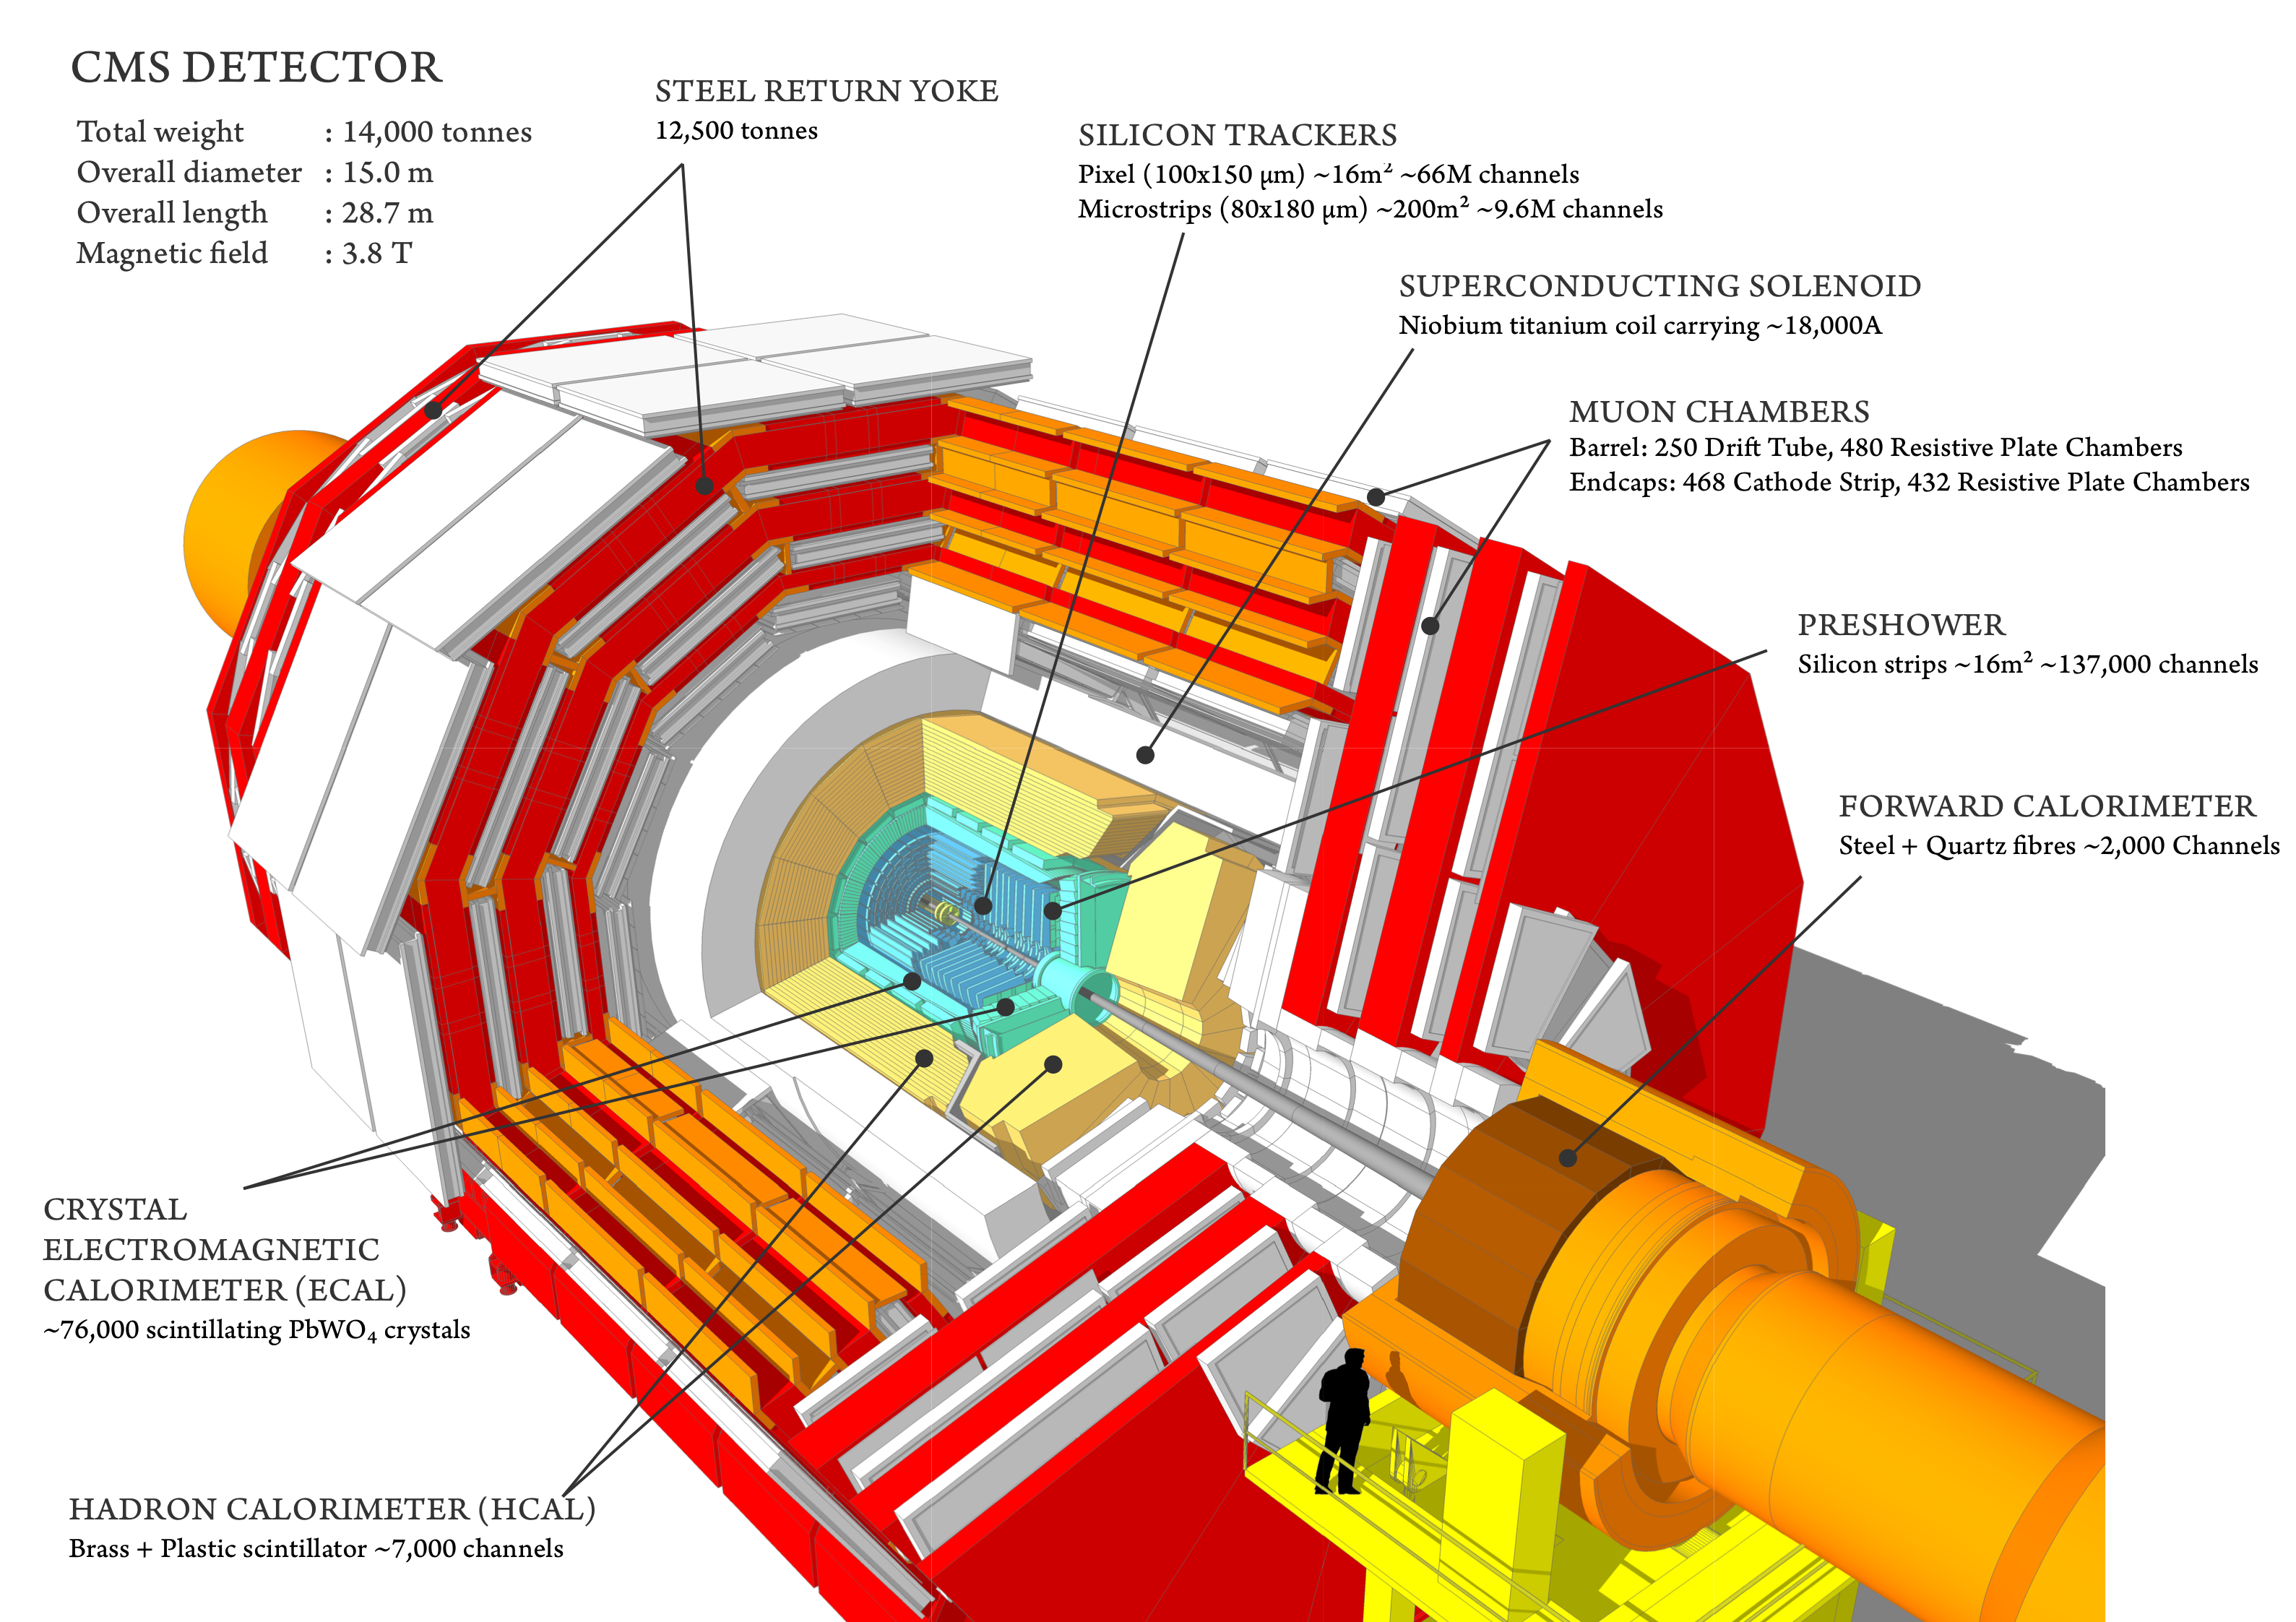
\includegraphics[width=1\textwidth]{figs/detector/cms3d}
\caption{Layout of the major components within the CMS detector. These are 
described in the text.}
\label{fig:cms3d}
\end{figure}
\begin{figure}
\centering
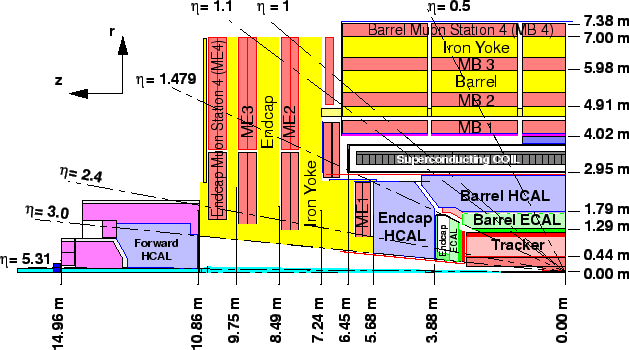
\includegraphics[width=0.8\textwidth]{figs/detector/cms2d.png}
\caption{One quarter cross-sectional view (in the $r$-$z$ plane) of the CMS 
detector, indicating lines of constant pseudorapidity and the dimensions of 
various components.}
\label{fig:cms2d}
\end{figure}

%Diagram.
%Overview of subdetectors. Magnet strength.
The tracker forms the first layer of the detector closest to the collision 
point. It is used to reconstruct the trajectories of charged particles within 
the magnetic field and measure their momenta. Following this is the 
electromagnetic calorimeter (ECAL), which is used to absorb and measure the 
energies of electrons and photons. The next layer is comprised of the hadronic 
calorimeter (HCAL), which detects the more penetrating hadrons. The 3.8~T 
superconducting solenoid surrounds the tracker and calorimeters. Muons are able 
to penetrate the magnet and calorimeters and are detected by the muon chambers, 
which are interspersed with the steel return yoke of the magnet in the 
outermost layer of the CMS enclosure.
TODO: one sentence on trigger and daq (see adam).

%Coordinate system. Pseudorapidity. Cylindrical radius r.
% phi measured from x axis
A right-handed coordinate system is defined with the origin at the interaction 
point. The $x$-axis lies horizontally towards the centre of the LHC ring, the 
$y$-axis points vertically upwards, and the $z$-axis points along the beam 
direction. An azimuthal angle $\phi$ is defined that lies in the transverse 
$x$-$y$ plane. The cylindrical radial coordinate is labelled $r$. A polar angle 
$\theta$ is measured from the $z$-axis and is related to 
pseudorapidity by $\eta = -\ln\left[\tan\left(\frac{\theta}{2}\right)\right]$.

\begin{comment}
The Compact Muon Solenoid (Fig. 1) is one of the two general purpose detectors,
along with ATLAS, at the LHC. It comprises a 13 m long, 4 T superconducting 
solenoid magnet within which lie a tracker, an electromagnetic calorimeter 
(ECAL) and a hadronic calorimeter (HCAL). Outside the magnet and within the 
return yoke lies the muon detection system.
The tracking system consists of an inner silicon pixel detector and an outer 
silicon microstrip tracker. The ECAL is constructed from crystals of lead 
tungstate and measures the energies of photons and electrons. The scintillation 
light produced by these particles as they pass through the crystals is detected 
by photodetectors. The HCAL consists of alternating brass absorbers and plastic 
scintillators. It surrounds the ECAL and detects the more penetrating hadrons. 
Muons are able to penetrate the magnet and calorimeters and are detected by 
chambers on the edge of the CMS enclosure. These consist of drift tubes and 
cathode strip chambers along with resistive plate chambers to provide a fast 
trigger response.
\end{comment}

TODO (maybe) Give extent (in radius) occupied by each subdetector as you go 
along.

\subsection{Tracker}
%How tracker works, ie electron-hole pairs (see Adam and MSci report).
%High radiation environment. Little material.
%Pixel tracker. (for vertices) r<20 cm
%Silicon strip tracker.
%TOB, TEC, etc. Their positions/extents.
%Momentum resolution, tracking efficiency, spatial resolution.
% follow MA and MSci report
The CMS tracker consists of a silicon pixel detector located closest to the 
interaction point ($r<20$~cm) and silicon strip detectors surrounding this. 
The more granular pixels are used to cope with the higher particle fluxes that 
are present near the interaction point, as well as to provide a precise vertex 
reconstruction, including secondary vertices from the decays of long-lived 
particles such as b-hadrons. At larger radii the particle flux is lower such 
that strip detectors can be used instead. There are a total of 66 million 
silicon pixels and 9.6 million silicon strips covering an area of about 
200~m$^2$. The arrangement of tracker modules is illustrated in 
Fig.~\ref{fig:tracker}.

The pixel detector comprises 3 barrel layers and 2 endcap layers. Each pixel is 
$100~\micro\metre\times150~\micro\metre$ in size. The spatial 
resolution is approximately $10~\micro\metre$ in the {$r$-$\phi$} plane and 
$20~\micro\metre$ in the $z$ direction.

The barrel section of the strip detector comprises the Tracker Inner Barrel 
(TIB) consisting of 4 layers, and the Tracker Outer Barrel (TOB) consisting of 
6 layers. The strips range in size from $10~\centi\metre\times80~\micro\metre$ 
in the TIB to $25~\centi\metre\times180~\micro\metre$ in the TOB. The endcap 
region of the strip detector is made up of the Tracker End Cap (TEC) consisting 
of 9 disks, and the 3 Tracker Inner Disks (TID) that lie between the TIB and 
the TEC.
%strips resolution ranges between 13-47 microns

The tracker is able to record a hit of a charged particle with $\pt>1$~GeV with 
an efficiency of over 99\%. The transverse momentum resolution 
$\frac{\Delta\pt}{\pt}$ is approximately 2\% for particles with $\pt = 100$~GeV.

%Diagram of layout.
\begin{figure}
\begin{center}
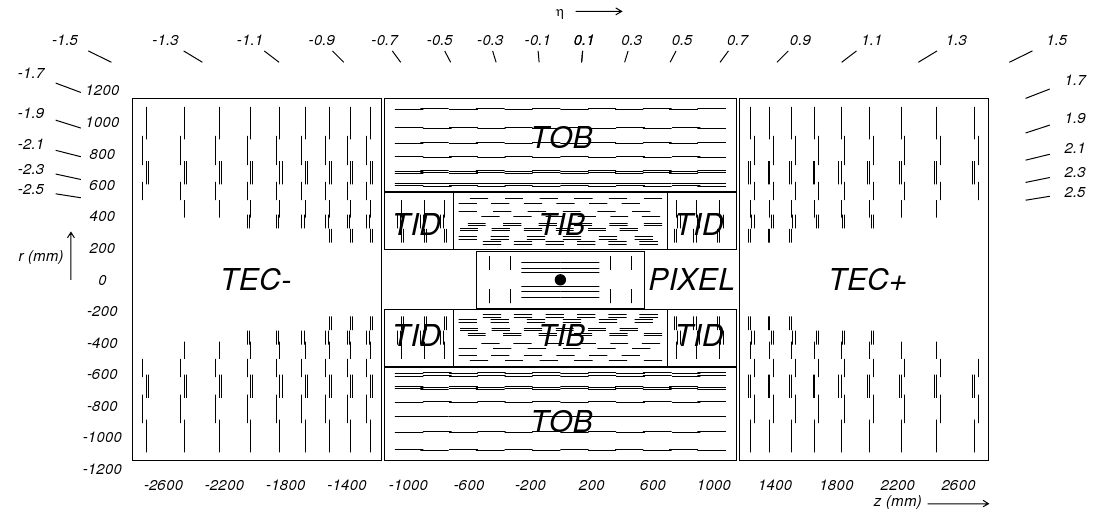
\includegraphics[width=0.8\linewidth]{figs/detector/tracker}
\end{center}
\caption{Schematic cross-sectional view (in the $r$-$z$ plane) of the CMS 
tracker~\cite{cms}. The tracker modules are indicated by the black line 
segments.}
\label{fig:tracker}
\end{figure}

\subsection{Electromagnetic calorimeter}

Designed to detect electrons and photons. Lead tungstate crystals.

EB. EE. Preshower.

Diagram of layout.

How ECAL works (ECAL shower, bremmstrahlung and pair production - see Adam and 
APP MSci course.)

Resolution formula (a+b+c).

\subsection{Hadronic calorimeter}

Designed to detect hadrons/jets. Brass and scintillating plastic. Photodiodes. 
HF. Fibres.

HB. HE. HO. HF

Diagram of layout.

How HCAL works (hadronic showers produce scintillation light - see Adam and APP 
MSci course.)

Resolution formula.

\subsection{Muon system}

Adam: As muons are heavier than electrons, they are minimally ionising and lose 
little energy through bremsstrahlung. They therefore mostly pass through the 
ECAL and HCAL. As muons are a key component of many electroweak decays, CMS has 
a dedicated muon system interleaved with the iron return yoke surrounding the 
solenoid.
 
DT (MB), CSC (ME), RPC.

Diagram of layout.

Momentum resolution 1\%.

\subsection{Magnet}

Just one or two short paragraphs.
See Marco-Andrea, Citron, Baber.

\subsection{Trigger and data acquisition}

% https://cms.cern/detector/computing-grid

40 MHz.

L1 trigger.

HLT.

%\subsection{Software and computing}
% CMSSW
Computing tiers.

\subsubsection{L1 trigger upgrade and my service work?}

Not sure yet. Look at Adam, Matt, Jad.

\section{Event reconstruction}
\label{sec:detector-reconstruction}

Intro: need to put together the things observed in the detector to reconstruct 
the objects.

Object reconstruction/identification (requires revision).
Tag and probe.
vertexing/tracking, btagging, PF, antikt.
PU subtraction, isolation, cross-cleaning.
MC corrections (JECs, PU, btagging, lepton ID, etc.).

Mention objects/working points used in analysis as you go along. Maybe summary 
table like Matt. Actually maybe include this in analysis chapter (see Adam).

\subsection{Tracks and vertices}

Combinatorial track finder (CTF), Kalman filter.

Primary vertex. PU vertices. Secondary/displaced vertices (b quarks) found in 
subsequent levels of reconstruction.

Efficiencies.

Isolated tracks? (when talking about analysis objects).

\subsection{Electrons and photons}
%\subsubsection{Tag and probe/corrections}

\subsection{Muons}

Global and tracker muons.

Define relative and mini-isolation.
Define pileup subtraction - effective rho area, delta beta?
(have a dedicate section like adam)

% page 27 https://arxiv.org/pdf/1502.02702.pdf
rho*Aeff, where rho is the median of the transverse energy density per unit 
area in 
the event [26] and Aeff is the area of the isolation region weighted by a 
factor that takes into account the dependence of the pileup transverse energy 
density on pseudorapidity. The effective areas have been determined in gamma + 
jet events.

\subsection{Particle flow algorithm}
Need to decide where to put this. Not clear on the connection between object 
reconstruction and particle flow.
Resources: Particle Flow paper, Particle Flow summary.

The tracks are extrapolated through the calorimeters, if they fall within the 
boundaries of one or several clusters, the clusters are associated to the 
track. The set of track and cluster(s) constitute a charged hadron and the 
building bricks are not considered anymore in the rest of the algorithm. The 
muons are identified beforehand so that their track does not give rise to a 
charged hadron. The electrons are more difficult to deal with. Indeed, due to 
the frequent Bremsstrahlung photon emission, a specific track reconstruction [3]
is needed as well as a dedicated treatment to properly attach the photon 
clusters to the electron and avoid energy double counting. Once all the tracks 
are treated, the remaining clusters result in photons in case of the 
electromagnetic calorimeter (ECAL) and neutral hadrons in the hadron 
calorimeter (HCAL). Once all the deposits

\subsection{Jets}

Briefly describe what a jet is (hadronisation, tight cone of particles [MA]).
antikt algorithm. Infrared and collinear safe.
Inputs are PF candidates. Pileup subtraction (not just here but for all 
objects).

\subsubsection{Correcting the energy of jets}
\label{sec:detector-jecs}
JECs. JER?

\subsubsection{b-tagging}
\label{sec:detector-btagging}
Identification of jets originating from bottom quarks.

see btagging CMSDAS Introduction.pdf
eg slide 11 how eff varies with pt and eta, ROC curves, etc.

\subsection{Energy sums and missing energy}

Define HT, MHT and MET. At some point (maybe near the beginning) explain why we 
use  the transverse plane (initial momentum is zero, whereas it isn't in the 
longitudinal plane).

Neutrinos do not interact in particle detectors, and therefore escape 
undetected. Their presence can be inferred by the momentum imbalance of the 
visible particles in an event. (this should be mentioned in overview of 
analysis in intro chapter).

Type-1 corrections.


\section{Simulation}
\label{sec:detector-simulation}

\textsc{MadGraph5}~\cite{madgraph}
\textsc{powheg}~\cite{powheg}
\textsc{pythia8}~\cite{pythia}
\textsc{geant4}~\cite{geant}

\begin{comment}
\section{Data sets}

See Nick. MA has this in the analysis chapter.
We use data collected by the CMS during certain runs, plus simulated data of 
background and signal processes.

\subsection{Collected data}

35.9 fb-1. 2016. (This would be mentioned in the intro anyway).
Show lumi delivered/collected vs time.
Triggers/Primary Datasets.
SR and Muon CRs.

Maybe keep this chapter general, just have section on MC simulation, and 
mention which specific data and MC samples elsewhere.

\subsection{Monte Carlo simulation}

Description of madgraph, pythia, GEANT.

MC simulation data sets.
(Grid of masses and ctau, couplings used) - no need to specify grid, couplings 
mentioned in simplified models section.
See paper.

Describe weights and xs/lumi normalisation?
\end{comment}